\documentclass{beamer}
\usefonttheme{serif}
\usepackage{amsmath} %数学公式
\usepackage{newtxtext,newtxmath} %新罗马
\usepackage{mathrsfs} %花体
\usepackage{amssymb} %空心
\usepackage{graphicx} %图片
\usepackage{float}
\usepackage[absolute,overlay]{textpos} %文本框
\usepackage{tikz} %tikz
\usepackage{booktabs}%三线表
\usepackage{multirow} %表格
\usepackage{siunitx} %SI单位
\usepackage{makecell} %表格里一对二
\usepackage{subfig}
\usepackage{caption}
\usepackage{tikz}
\usepackage{threeparttable}
\usetikzlibrary{arrows}
\setbeamertemplate{caption}[numbered]



\captionsetup[figure]{font=scriptsize,labelfont=scriptsize,labelformat={default},labelsep=period,name={Fig}}
\captionsetup[table]{font=scriptsize,labelfont=scriptsize,labelformat={default},labelsep=period,name={Tab}}


\title{Electrostatic Interactions in the Post-Ewald Era: Theoretical Insights and Machine Learning Treatments}
\author{ \Large{Yihao Zhao }  }
\institute{Shandong University \\
	Qingdao Institute for Theoretical and Computational Sciences(QiTCS)\\ \textit{zhaoyihao@protonmail.com}}


\begin{document}
	
	\begin{frame}
		\titlepage
	\end{frame}
	
	\begin{frame}
		\frametitle{Electrostatic interactions in periodic systems }
		
		\footnotesize
		
		\vspace{-2pt}
		
		Periodic Boundary Conditions(PBC)\footnote{M. P. Allen and D. J. Tildesley, \textit{Computer Simulation of Liquids}, 2nd ed., Oxford University Press, 2017}
		
		\vspace{13pt}
		
		\begin{textblock*}{5cm}(3cm,1.9cm)
			\includegraphics[width=0.3\linewidth]{./figure/PBC/noPBC.pdf}
		\end{textblock*}
		
		\begin{textblock*}{5cm}(3.8cm,2.5cm)
			\centering
			\LARGE $\longrightarrow$
		\end{textblock*}
		
		\begin{textblock*}{5cm}(8cm,0.8cm)
			\includegraphics[width=0.7\linewidth]{./figure/PBC/PBC.pdf}
		\end{textblock*}
		
		\vspace{2cm}
		
		Electrostatic Energy Calculation Under PBC:
		\[
		E= \dfrac{1}{2} \sum_{i=1}^{\infty} \sum_{j=1, j\ne i}^{\infty} q_iq_j \dfrac{1}{r_{ij}} \quad \longrightarrow \quad 
		E= \dfrac{1}{2} \sum_{i=1}^{N} \sum_{j=1}^{N} q_iq_j \bigg{(}\sum_{\mathbf{n}\in \mathbb{Z}^3}\!' \dfrac{1}{|\mathbf{r}_{ij}+\mathbf{n}\mathbf{L}|} \bigg{)}
		\]
		
		The periodic extension of the Coulomb potential leads to a \textbf{conditionally convergent} series.   
		\begin{align*}
			S_A =& 1 - \dfrac{1}{2} + \dfrac{1}{3} - \dfrac{1}{4} + \dfrac{1}{5} + \cdots  = \ln 2 \\
			S_A =& (1 - \dfrac{1}{2}) - \dfrac{1}{4} + (\dfrac{1}{3} - \dfrac{1}{6} ) - \dfrac{1}{8} + \cdots  
			=& \dfrac{1}{2}(  1 - \dfrac{1}{2} + \dfrac{1}{3} - \dfrac{1}{4} + \dfrac{1}{5} + \cdots  ) = \dfrac{1}{2}\ln 2 
		\end{align*}
	\end{frame}		
	%%%%%%%%%%%%%%%%%%%%%%%%%%%%%%%%%%%%%%%%%%%%%%%%%%%%%%%%%%%%%%%%%%		
	\begin{frame}
		\frametitle{Ewald Summation Method}
		
		\footnotesize
		
		\vspace{-7pt}
		
		P. P. Ewald splits the Coulomb potential\footnote{P. P. Ewald, \textit{Ann. Phys.} \textbf{64}, 253 (1921)}
		\begin{textblock*}{5cm}(2cm,1.9cm) % 调整位置
			\[
			\dfrac{1}{r} = \dfrac{\text{erfc}(\alpha r)}{r} + \dfrac{\text{erf}(\alpha r)}{r}
			\] 
		\end{textblock*}  
		
		\vspace{1.4cm}
		Traditional Ewald energy:
		\begin{textblock*}{10cm}(1cm,3.25cm)  
			\begin{align}
				E =	&\dfrac{1}{2}\sum_{\mathbf{n} \in \mathbb{Z}^3}\sum_i^N\sum_j^N \!' q_iq_j\dfrac{\text{erfc}(\alpha|\mathbf{r}_{ij}+\mathbf{n}\mathbf{L}|) }{|\mathbf{r}_{ij}+\mathbf{n}\mathbf{L}|}-\dfrac{\alpha}{\sqrt{\pi}}\sum_i^N q_i^2 \quad \text{$R$-space sum}  \notag \\	
				+ & \dfrac{1}{2V} \sum_i^N \sum_j^N q_i q_j  \sum_{\mathbf{k}\ne 0}\dfrac{4\pi}{k^2}e^{-\frac{k^2}{4\alpha^2}}
				e^{i\mathbf{k}\cdot \mathbf{r}_{ij}} 		
				\quad \text{$k$-space sum}  \notag 	
			\end{align}	   	
		\end{textblock*}
		
		\vspace{3cm}
		Remaining boundary term :
		\begin{equation*}
			E^{IB}=\dfrac{1}{2V} \sum_i^N \sum_j^N q_i q_j  \lim\limits_{\mathbf{k} \to 0}\dfrac{4\pi}{k^2}e^{-\dfrac{k^2}{4\alpha^2}}
			e^{i\mathbf{k}\cdot \mathbf{r}_{ij}  } 	
		\end{equation*}
		
		\begin{textblock*}{10cm}(5.5cm,4.2cm)  
			\begin{figure}[h]
				\centering
				\includegraphics[width=0.4\linewidth]{./figure/erf/errorFunc.pdf}
				%	\caption{error function erf($\cdot$) and \\	   		
					%	complementary error function erfc($\cdot$)}
			\end{figure}
		\end{textblock*}
		
		\begin{textblock*}{10cm}(4.9cm,1cm)  
			\begin{figure}[h]
				\centering
				\includegraphics[width=0.5\linewidth]{./figure/Gauss/Gauss.pdf}
				%	\caption{error function erf($\cdot$) and \\	   		
					%	complementary error function erfc($\cdot$)}
			\end{figure}
		\end{textblock*}
		
		The Ewald method is the \textbf{gold standard} in electrostatic computation.
	\end{frame}
	
	%%%%%%%%%%%%%%%%%%%%%%%%%%%%%%%%%%%%%%%%%%%%%%%%%%%%%%%%%%%%%%%%%%	
	%%%%%%%%%%%%%%%%%%%%%%%%%%%%%%%%%%%%%%%%%%%%%%%%%%%%%%%%%%%%%%%
	%%%%%%%%%%%%%%%%%%%%%%%%%%%%%%%%%%%%%%%%%%%%%%%%%%%%%%%%%%%%%%%%%%		
	\begin{frame}
		\frametitle{ The Post Ewald Era}		
		\small 
		
		Pitfalls and Misconceptions of the Ewald Method:
		
		\begin{itemize}
			\item The physical picture of the $k$-space sum is not intuitive.
			\item Inherently tied to PBC, which can affect simulation outcomes.
			\item Low computational efficiency $\mathscr{O}(N^2)$.
			\item Contains an arbitrary parameter $\alpha$.
		\end{itemize}
		
		\vspace{0.8cm}
		
		Therefore, electrostatic energy calculations have diverged into two main directions:
		
		\begin{itemize} 
			\item Abandoning Ewald's concept, developing purely real-space electrostatics.
			\item Building upon Ewald's concept, focusing on computational efficiency.
		\end{itemize}
		
		
	\end{frame}
	
	
	%%%%%%%%%%%%%%%%%%%%%%%%%%%%%%%%%%%%%%%%%%%%%%%%%%%%%%%%%%%%%%%%%%%%%%%
	
	\begin{frame}
		\frametitle{ I .  A Unified Theoretical Framework}		
		
		
		Abandoning Ewald's concept and developing purely real-space electrostatics introduces the following issues:
		\vspace{0.6cm}
		
		\begin{itemize} 
			\item Can these new electrostatic interactions correctly reproduce the physical properties they govern? 
			\vspace{0.3cm}
			\item Can this correctness be determined directly from their functional forms?
		\end{itemize}
		
		\vspace{0.6cm}
		Thus, a unified  theoretical framework connecting \textbf{functional forms} and \textbf{physical properties} is necessary\footnote{Y. Zhao and Z. Hu, \textit{J. Chem. Theory Comput.} \textbf{21}, 5916 (2015)}.
	\end{frame}

	%%%%%%%%%%%%%%%%%%%%%%%%%%%%%%%%%%%%%%%%%%%%%%%%%%%%%%%%%%%
	%%%%%%%%%%%%%%%%%%%%%%%%%%%%%%%%%%%%%%%%%%%%%%%%%%%%%%%%%%%%%%%%5
	\begin{frame}
		\frametitle{ I .  The Interaction Benchmark and Its Fundamental Defect}
				
		\begin{columns}[T]
			
			\begin{column}{0.5\textwidth}
				\textbf{The Ideal Benchmark}
				\vspace{0.5em}
				
				\footnotesize
				The complete electrostatic interaction is the fundamental benchmark for any physical property:
				\vspace{-0.5em}	
				\footnotesize
				\begin{equation*}
					u_{\text{pair}}(\mathbf{r}) = \dfrac{1}{r} + \sum_{\mathbf{n} \ne 0} \bigg{(} \dfrac{1}{|\mathbf{r} + \mathbf{nL}|} - \dfrac{1}{|\mathbf{n}\mathbf{L}|} \bigg{)} 
				\end{equation*}
				
				Termwise Rearrangement:
				\begin{equation*}
					u_{\text{pair}}^{\text{red}}(\mathbf{r}) = u_{\text{pair}}(\mathbf{r})  ,\quad
					u_{\text{pair}}^{\text{blue}}(\mathbf{r}) = u_{\text{pair}}(\mathbf{r} - L_x\mathbf{e}_x)   
				\end{equation*}
				
				
				Energy of an Identical Charge in an Identical Lattice:
				\begin{equation*}
					\Delta u \sim L^{-1} \neq 0
				\end{equation*}
				The benchmark is non-unique.
			\end{column}% 
			
			
			\begin{column}{0.5\textwidth}
				\textbf{An Intrinsic Physical Defect}
				\vspace{-0.5em}
				
				\footnotesize
				
				\centering 
				\begin{figure}
					\centering
					\includegraphics[width=0.5\linewidth]{./figure/lattice/cell.pdf}
				\end{figure}	
				\vspace{-0.9em}
				Reclassification of unit cells:
				\vspace{-0.5em}
				\begin{figure}
					\centering
					\includegraphics[width=0.9\linewidth]{./figure/lattice/lattice.pdf}
				\end{figure}
				\vspace{-0.5em}
			\end{column}
		\end{columns} %
		
		\noindent\rule{\textwidth}{0.4pt}
		\centering
		\small
		\textbf{
			Therefore, electrostatic interactions have a rigorously correct form, \\ but it is not directly usable in practical simulations.}
	\end{frame} % 
	%%%%%%%%%%%%%%%%%%%%%%%%%%%%%%%%%%%%%%%%%%%%%%%%%%%%%%%%%%%
	\begin{frame}
		\frametitle{I . Traditional Ewald Interaction }
		\footnotesize 
		
		\begin{textblock*}{8cm}(0.3cm,0.5cm)  
			\begin{equation*}
				u_{\text{pair}}^{tf}(\mathbf{r}) = \dfrac{\mathrm{erfc}(\alpha r)}{r} + \sum_{\mathbf{n}\ne 0} \bigg{(}\dfrac{\mathrm{erfc}(  \alpha|\mathbf{r}+\mathbf{n}\mathbf{L}|)}{|\mathbf{r}+\mathbf{n}\mathbf{L}|} - \dfrac{\mathrm{erfc}(  \alpha|\mathbf{n}\mathbf{L}|)}{|\mathbf{n}\mathbf{L}|}\bigg{)} + \dfrac{2\alpha}{\sqrt{\pi}} 
				+\dfrac{1}{V} \sum_{\mathbf{k}\ne 0} \dfrac{4\pi}{k^2} e^{-\dfrac{k^2}{4\alpha^2}}(e^{i\mathbf{k}\cdot \mathbf{r}} - 1) 
			\end{equation*}
		\end{textblock*}
		
		\begin{textblock*}{8cm}(0.3cm,2cm)  
			\begin{align*}
				u^{\text{ib}}_{\text{pair}}(\mathbf{r}) =& -\dfrac{2\pi}{V} \lim\limits_{\mathbf{k} \to 0} \dfrac{(\mathbf{k}\cdot \mathbf{r})^2}{|\mathbf{k}^2|} 
				= \dfrac{1}{2V} \lim\limits_{\Omega \to \infty} \oint_{\partial \Omega} dS \,\mathbf{n} \cdot  \bigg{[}\mathbf{r} \cdot\bigg{(}\mathbf{r}\cdot \nabla_{\mathbf{a}} \dfrac{1}{|\mathbf{a}|}\bigg{)} \bigg{]}  \\
				=& 
				\begin{cases}			
					\text{cube-shaped} \, \Omega 	& \overset{\;+\; u^{tf}_{\text{pair}} \;}{\scalebox{1.5}{$\longrightarrow$}}  u^{ib, cube}_{\text{pair}}(\mathbf{r}) = u_{\text{pair}}^{tf}(\mathbf{r}) -   \dfrac{2\pi}{3V} r^2 \\
					\text{plate-shaped} \, \Omega &  \overset{\;+\; u^{tf}_{\text{pair}} \;}{\scalebox{1.5}{$\longrightarrow$}} u^{ib, plate}_{\text{pair}}(\mathbf{r}) = u_{\text{pair}}^{tf}(\mathbf{r}) -   \dfrac{2\pi}{V} z^2 \\
					\text{other shape} & \overset{\;+\; u^{tf}_{\text{pair}} \;}{\scalebox{1.5}{$\longrightarrow$}} \, u^{ib, shape}_{\text{pair}}(\mathbf{r}) = u_{\text{pair}}^{tf}(\mathbf{r}) + \cdots
				\end{cases}
			\end{align*}
		\end{textblock*}
		\begin{textblock*}{8cm}(0.3cm,6.1cm)  
			\begin{equation*}
				u_{\text{pair}}^{tf}(\mathbf{r})  : \text{  a rearrangement of    } \quad  \dfrac{1}{r} + \sum_{\mathbf{n}\in \mathbb{Z}^3, \mathbf{n} \ne 0}^{\infty} \bigg{(}\dfrac{1}{|\mathbf{r}+\mathbf{n}\mathbf{L}|} - \dfrac{1}{|\mathbf{n}\mathbf{L}|} \bigg{)} - u^{ib}_{\text{pair}}(\mathbf{r})
			\end{equation*}
		\end{textblock*}
		\begin{textblock*}{10cm}(6cm,1.7cm)  
			\begin{figure}[h]
				\centering
				\includegraphics[width=0.3\linewidth]{./figure/shaped/cube.pdf}
			\end{figure}
		\end{textblock*}
		\begin{textblock*}{10cm}(6.2cm,4.8cm)  
			\begin{figure}[h]
				\centering
				\includegraphics[width=0.25\linewidth]{./figure/shaped/plate.pdf}
			\end{figure}
		\end{textblock*}
		\begin{textblock*}{10cm}(0.3cm,7.7cm)     
			\noindent\rule{\textwidth}{0.4pt}
			\centering
			\small
			\textbf{
				The Ewald interaction class results from a definitive summation order mathematically, and its form embodies the crystal's tiling rules (shape) physically.}
		\end{textblock*}
	\end{frame}
	%%%%%%%%%%%%%%%%%%%%%%%%%%%%%%%%%%%%%%%%%%%%%%%%%%%%%%%%%%
	\begin{frame}
		\frametitle{I . Purely Real-Space Interactions without k-Space  }
		\footnotesize 
		
		\begin{columns}[T]
			
			\begin{column}{0.5\textwidth}
				\vspace{0cm}
				\textbf{Angular-Averaged Ewald interaction}\footnotemark[4]
				\vspace{-0.3em}
				\begin{align*}
					u_{\text{pre-aa}}(r) =& \dfrac{1}{4\pi} \int_{0}^{2\pi} d\phi \int_{0}^{\pi} d\theta \sin \theta \, u_{\text{pair}}^{tf}(\mathbf{r})   \\     
					=&
					\begin{cases}
						\dfrac{1}{r} + \dfrac{r^2}{2r_m^3} - \dfrac{3}{2r_m} & r \le r_m \\
						0& r > r_m
					\end{cases} 
				\end{align*} 
				\begin{textblock*}{3cm}(0.5cm,3.5cm)  
					\begin{figure}
						\centering
						\includegraphics[width=0.7\linewidth]{./figure/cubeball/cubeball.pdf}
					\end{figure}
				\end{textblock*} 
				\begin{textblock*}{3cm}(3cm,4.5cm)  
					\begin{equation*}
						\dfrac{4\pi}{3}r_m^3 = V_{\text{cell}}
					\end{equation*}
				\end{textblock*} 
				
				\vspace{1.8cm}
				It's periodic extension constitutes:
				\vspace{-0.8em}
				\begin{equation*}
					u_{\text{pair}}^{aa} (\mathbf{r})=  u_{\text{pre-aa}}(r) + \sum_{\mathbf{n}\ne 0}^{\infty} u_{\text{pre-aa}}(|\mathbf{r} + \mathbf{nL}|) 
				\end{equation*}
				\textbf{We provide a rigorous derivation in a single step, that is, starting from the infinite series form.}
			\end{column}% 
			
			
			\begin{column}{0.5\textwidth}
				
				\textbf{Zero-Multipole interaction}\footnotemark[5]
				\vspace{-0.5em}
				\begin{equation*}
					E_{\text{ZM}} = \dfrac{1}{2} \sum_{i=1}^N \sum_{j\in \mathscr{M}_i^{(l)} } q_iq_j u(\mathbf{r}_{ij}) 
				\end{equation*}
				
				\begin{textblock*}{3cm}(6cm,2.7cm)  
					\begin{figure}
						\centering
						\includegraphics[width=0.8\linewidth]{./figure/zmball/zmball.pdf}
					\end{figure} 
				\end{textblock*} 
				
				\begin{textblock*}{3cm}(8.8cm,3.2cm)  
					$\mathscr{M}_i^{(l)}$: the set of charge indices such that the moments up to the $l$-th order in its union with $i$ are zero.
				\end{textblock*}
				
				\vspace{2.1cm}
				\begin{equation*}
					E_{\text{ZM}}
					\approx \dfrac{1}{2} \sum_{i=1}^N \sum_{j \ne i, r_{ij} < r_c }  q_iq_j u_{\text{pair}}^{zm, l} (r_{ij}) 
				\end{equation*}
				\begin{equation*}
					u_{\text{pair}}^{zm, l} \equiv  \text{it's periodic extension}
				\end{equation*}    	
				\textbf{A derivation error exists after approximation, but not for orders $l \le 2$ and below.}
			\end{column}
		\end{columns} 
		
	    \footnotetext[4]{E. Yakub and C. Ronchi, \textit{J. Chem. Phys.} \textbf{119}, 11556 (2003)}
	    \footnotetext[5]{I. Fukuda, \textit{J. Chem. Phys.} \textbf{139}, 174107 (2013)}
	\end{frame}
	%%%%%%%%%%%%%%%%%%%%%%%%%%%%%%%%%%%%%%%%%%%%%%%%%%%%%%%%%%%%
	\begin{frame}
		\frametitle{I . Dielectric Response and Boundary Term Form}
		\footnotesize 
		\begin{textblock*}{7cm}(0.5cm,0.7cm)  
			\begin{figure}[t]
				\centering
				\includegraphics[width=\linewidth]{./figure/chargepair/chargepair.pdf}
			\end{figure}
		\end{textblock*}
		
		\begin{textblock*}{4cm}(8cm,1.2cm) 
			Linear response :
			\begin{equation*}
				\mathbf{M}_{\text{ind}}/V = \varepsilon_0 (\epsilon - 1) (\mathbf{E}_{\text{app}} -  \mathbf{E}_{\text{pol}} )
			\end{equation*}
			Depolarization field :  		
			\begin{equation*}
				\mathbf{E}_{\text{pol}} = -\gamma \mathbf{M}_{\text{ind}}/V \varepsilon_0
			\end{equation*}
		\end{textblock*}	
		
		\begin{textblock*}{10cm}(-0.1cm,3.5cm) 
			\begin{equation*}
				\gamma = 
				\begin{cases}
					1/3  & \text{cube} \Leftrightarrow \text{ib, cube  } \quad   u^{ib, cube}_{\text{pair}} \, \rightarrow \quad	\varepsilon_0\frac{\mathbf{M}_{\text{ind}}^{ib,cube} }{3V}= \frac{ (\epsilon - 1)} {(\epsilon+2)}\mathbf{E}_{\text{app}} \\
					1    & \text{plate} \Leftrightarrow \text{ib, plate  } \quad   u^{ib, plate}_{\text{pair}}
					\rightarrow \quad	\varepsilon_0\frac{\mathbf{M}_{\text{ind}}^{ib, plate}}{V}= \frac{ (\epsilon - 1)} {\epsilon}\mathbf{E}_{\text{app}} \\
					0 & \text{no-boundary} \Leftrightarrow \text{tf }  \quad   u^{tf}_{\text{pair}}   \,\, \,\, \rightarrow \quad \quad  \frac{\mathbf{M}_{\text{ind}}^{tf}}{V}  =  \varepsilon_0(\epsilon - 1) \mathbf{E}_{\text{app}} 
				\end{cases}
			\end{equation*}
		\end{textblock*}
		
		\begin{textblock*}{4cm}(10cm,4.3cm) 
			Similarly for \\
			other shapes ($\gamma$).
		\end{textblock*}   
		
		\begin{textblock*}{10cm}(1cm,5.6cm)  
			\begin{table}[h]
				\centering    		
				\resizebox{\textwidth}{!}{%	
					\begin{threeparttable}     		
						\begin{tabular}{*{8}{c}}
							\toprule
							\multirow{2}{*}{\makecell{ model \& \\spring \\constants }} & \multirow{2}{*}{\makecell{$E_{\text{app}}(\mathrm{V}/\text{\AA})$}} & \multicolumn{2}{c}{tf} & \multicolumn{2}{c}{ib, plate} & \multicolumn{2}{c}{ib, cube} \\
							\cmidrule(lr){3-4} \cmidrule(lr){5-6} \cmidrule(lr){7-8}
							& & $\dfrac{M_{\text{ind}}^{tf} }{V\epsilon_0}(\mathrm{V}/\text{\AA})$ & $\epsilon_{\infty}$ & $\dfrac{{M}_{\text{ind}}^{ib,plate}}{V\epsilon_0}(\mathrm{V}/\text{\AA})$ & $\epsilon_{\infty}$ & $\dfrac{{M}_{\text{ind}}^{ib,cube}}{V\epsilon_0}(\mathrm{V}/\text{\AA})$ & $\epsilon_{\infty}$ \\
							\midrule    			
							\multirow{2}{*}{ion, $\kappa$} & 0.1 & 0.03654  & \multirow{2}{*}{1.3654}  &  0.02751& \multirow{2}{*}{1.3794} & 0.03369 & \multirow{2}{*}{1.3795} \\ 
							& 0.2 &  0.07308 &   &  0.05501 &  &  0.06738 & \\  \cmidrule(lr){2-8}                                				
							\multirow{2}{*}{mol, $\kappa$} & 0.1 & 0.03075  & \multirow{2}{*}{1.3075}  &  0.02352& \multirow{2}{*}{1.3075} & 0.02789 & \multirow{2}{*}{1.3075} \\ 
							& 0.2 & 0.06150  &   & 0.04704  &   &  0.05579 & \\
							\bottomrule
						\end{tabular}
				\end{threeparttable}}
			\end{table}
		\end{textblock*}
		
		
		
		\vspace{7.5cm}
		\noindent\rule{\textwidth}{0.4pt}
		\centering
		\small
		\textbf{We began by establishing  Geometric Shape is physically equivalent to Lattice Tiling Rule } 
	\end{frame}
	%%%%%%%%%%%%%%%%%%%%%%%%%%%%%%%%%%%%%%%%%%%%%%%%%%%%%%%%%%%%%%%%
	\begin{frame}
		\frametitle{I . Dielectric Response and Boundary Term Form}
		\footnotesize 
		
		\begin{textblock*}{4cm}(0.8cm,1.2cm) 
			
			Under adiabatic : 
			\begin{align*}
				&H_{\mathbf{E}}( \bar{\mathbf{f}}, \mathbf{E} )  =  H_0( \bar{\mathbf{f}}, \bar{\mathbf{e}}_0(\bar{\mathbf{f}}, \mathbf{E} )  ) - \mathbf{E}\cdot \mathbf{M}(\bar{\mathbf{f}}, \mathbf{E}) \\
				&\mathbf{M}(\mathbf{E}) = \dfrac{1}{Q(\mathbf{E})} \int  	\mathbf{M}(\bar{\mathbf{f}}, \mathbf{E}  )  e^{-\beta H_{\mathbf{E}}( \bar{\mathbf{f}}, \mathbf{E} )} d \bar{\mathbf{f}} 
			\end{align*}
		\end{textblock*}
		
		\begin{textblock*}{2cm}(2.6cm,3cm)  
			\begin{center}
				$\Downarrow$ 
			\end{center}
		\end{textblock*}
		
		\begin{textblock*}{8cm}(-0.5cm,3.4cm)  
			\begin{equation*}
				\dfrac{\partial \mathbf{M}(\mathbf{E})}{\partial \mathbf{E}} = \langle\dfrac{\partial\mathbf{M}(\bar{\mathbf{f}}, \mathbf{E}  ) }{\partial \mathbf{E} } \rangle + \beta \langle \mathbf{M}^2(\bar{\mathbf{f}}, \mathbf{E}  )  \rangle 
				-\beta \langle \mathbf{M}(\bar{\mathbf{f}}, \mathbf{E}  )  \rangle^2  
			\end{equation*}
		\end{textblock*}
		
		\begin{textblock*}{8cm}(-0.5cm,4cm)  
			\begin{center}
				\begin{equation*}
					\partial \mathbf{M} = \mathbf{M}_{\text{ind}} 
					\quad \Downarrow \quad 
					\partial \mathbf{E} = \mathbf{E}_{\text{app}}
				\end{equation*}
			\end{center}
		\end{textblock*}
		
		\begin{textblock*}{8cm}(0.1cm,5.4cm)  
			\begin{equation*}
				\beta	\dfrac{  \langle \mathbf{M}^2 \rangle - \langle \mathbf{M} \rangle^2 }{\varepsilon_0 V} = 
				\begin{cases}
					\dfrac{\epsilon - 1 }{\epsilon+2} - \dfrac{\epsilon_{\infty} - 1 }{\epsilon_{\infty}+2},\quad&
					u^{ib, cube}_{\text{pair}}  \\[6pt]
					\dfrac{\epsilon - 1 }{\epsilon} - \dfrac{\epsilon_{\infty} -1 }{\epsilon_{\infty}} ,\quad&
					u^{ib, plate}_{\text{pair}}\\[6pt]
					\epsilon - \epsilon_{\infty} 
					,\quad
					&u^{tf}_{\text{pair}} \\[6pt]
					\cdots ,\quad& u^{other-shape}_{\text{pair}}
				\end{cases}
			\end{equation*}
		\end{textblock*}		
		
		\begin{textblock*}{6cm}(6.5cm,0.7cm)  
			\begin{figure}[h]
				\centering
				\includegraphics[width=\linewidth]{./figure/Mfluct/Mfluct.pdf}
			\end{figure}
		\end{textblock*}
		
		\begin{textblock*}{5cm}(8cm,5.5cm) 
			• Unification of PBC dielectric response with macroscopic theory. \\ [5pt]
			• Elimination of artifacts in the traditional reaction field (RF)\footnotemark[6]\footnotemark[7]. \\ [10pt]
			In classical MD, $\epsilon_{\infty} = 1$.
		\end{textblock*}  
		
		\footnotetext[6]{S. W. de Leeuw and E. R. Smith, \textit{Proc. R. Soc. Lond. A} \textbf{373}, 57 (1980)}
		\footnotetext[7]{D. Frenkel and B. Smit, \textit{Understanding Molecular Simulation}, Academic Press, 2001}
		
	\end{frame}
	%%%%%%%%%%%%%%%%%%%%%%%%%%%%%%%%%%%%%%%%%%%%%%%%%%%%%%%%%%%%%%%
	\begin{frame}
		\frametitle{I . Dielectric Response and Boundary Term Form}
		\footnotesize
		
		\begin{textblock*}{8cm}(1cm,7cm)  
			\textbf{	First property-form link: } \\  [5pt  ]
			
			
			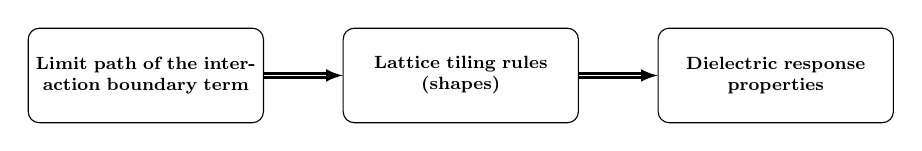
\begin{tikzpicture}[
				node style/.style={
					draw, 
					rounded corners, 
					align=center,
					minimum width=2.5cm,   
					minimum height=1.5cm,   
					font=\footnotesize,     
					text width=3.5cm,     
					fill=none
				},
				>=latex,
				scale=0.8,                 
				transform shape             
				]
				
				
				\node[node style] (node1) at (0,0) 
				{\textbf{Limit path of the interaction boundary term}};
				
				\node[node style] (node2) at (5,0) 
				{\textbf{Lattice tiling rules \\
						(shapes)}};
				
				\node[node style] (node3) at (10,0)    
				{\textbf{Dielectric response\\properties}};
				
				
				\draw[->, thick,double] (node1) -- (node2);
				\draw[->, thick,double] (node2) -- (node3);
				
			\end{tikzpicture}
		\end{textblock*}
		
		\begin{textblock*}{6cm}(0.5cm,1.2cm)  
			\begin{itemize}
				\item[$\bullet$] zm, 0: Non-zero dipole in cutoff $\rightarrow$ resembles IB (induces $E_{\text{pol}}$).
				\item[$\bullet$] zm, 2: Potential deviates from $1/r$, but converges with increasing $r_c$.
				\item[$\bullet$] aa : Artificial dipole correlation ($r_m > L/2$).
				\item[$\bullet$] $\Rightarrow$Accurate dipole fluctuation: zm, 1 only.
			\end{itemize}
		\end{textblock*}
		
		\begin{textblock*}{4cm}(1.5cm,5.2cm)  
			\begin{align*}
				u_{\text{pair}}^{zm,0} (r) =&  \dfrac{1}{r} - \dfrac{1}{r_c} \qquad (r \le r_c)  
			\end{align*}
		\end{textblock*}
		
		\begin{textblock*}{4cm}(6.8cm,4.7cm)  
			\begin{align*}
				u_{\text{pair}}^{zm,1} (r) =&  \dfrac{1}{r} + \dfrac{r^2}{2r_c^3} - \dfrac{3}{2r_c} \qquad (r \le r_c) \\
				u_{\text{pair}}^{zm,2} (r) =&  \dfrac{1}{r} - \dfrac{15}{8r_c} + \dfrac{5 r^2}{4r_c^3} -  \dfrac{3r^4}{8r_c^5} \qquad (r \le r_c) 
			\end{align*}
		\end{textblock*}
		
		\begin{textblock*}{6cm}(6.5cm,0.7cm)  
			\begin{figure}[h]
				\centering
				\includegraphics[width=\linewidth]{./figure/mdzm_aaMfluct/mdzm_aaMfluct.pdf}
			\end{figure}
		\end{textblock*}
		
	\end{frame}
	%%%%%%%%%%%%%%%%%%%%%%%%%%%%%%%%%%%%%%%%%%%%%%%%%%%%%%%%%%%%%%%%%%%%%%%%%
	\begin{frame}
		\frametitle{I .  Long-Range Correlation and Order of Divergence}
		\footnotesize 
		\begin{textblock*}{4cm}(0.8cm,1.2cm) 			
			Ornstein-Zernike : 
			\begin{equation*}
				h(\mathbf{r}_{12}) = c(\mathbf{r}_{12}) + \rho \int c(\mathbf{r}_{13}) h(\mathbf{r}_{32}) \, d \mathbf{r}_3 
			\end{equation*}
		\end{textblock*}
		
		\begin{textblock*}{2cm}(2.6cm,1.8cm)  
			\begin{center}
				\begin{equation*}
					\Downarrow \quad 
					\text{$k$-space}
				\end{equation*}
			\end{center}
		\end{textblock*}
		
		\begin{textblock*}{8cm}(-0.5cm,3.0cm)  
			\begin{equation*}
				S_{qq}(\mathbf{k}) = \dfrac{1}{V} \sum_{i=1}^N \sum_{j=1}^N q_i q_j \langle e^{i\mathbf{k}\cdot \mathbf{r}} \rangle  
			\end{equation*}
		\end{textblock*}
		
		\begin{textblock*}{8cm}(0.5cm,3.5cm)  
			\begin{center}
				\begin{equation*}
					\Downarrow \quad \text{Debye-Hückel approx}
				\end{equation*}
			\end{center}
		\end{textblock*}
		
		\begin{textblock*}{8cm}(-0.2cm,4.8cm)  
			\begin{equation*}
				S_{qq}(\mathbf{k}) =\dfrac{k^2I }{k^2 + \kappa_{\text{DH}}^2} 
				=  \dfrac{k_B T \varepsilon_0 }{\lambda_{\text{DH}}^2+ 1/k^2}  \quad \text{at small $k$}
			\end{equation*}
		\end{textblock*}		
		
		\begin{textblock*}{6cm}(1.1cm,6.5cm)  
			The correct order of divergence reflects whether a conductor can \textbf{fully screen} an external electric field (Stillinger-Lovett 2nd-moment condition\footnotemark[8]).
		\end{textblock*}
		
		\begin{textblock*}{6cm}(6.5cm,0.7cm)  
			\begin{figure}[h]
				\centering
				\includegraphics[width=\linewidth]{./figure/mdSqq/mdSqq.pdf}
			\end{figure}
		\end{textblock*}
		
		\begin{textblock*}{6cm}(7cm,6cm) 
			Other interactions only replacing $\mathscr{F}[1/r]$\footnotemark[9]:
		\end{textblock*}  
		\begin{textblock*}{5cm}(7.5cm,6.3cm) 
			
			\begin{equation*}
				\dfrac{\beta}{\varepsilon_0} \,\dfrac{S_{qq}(\mathbf{k})}{k^2}=
				\dfrac{1}{ \lambda_{\text{DH}}^2k^2 +  \varepsilon_0 k^2\mathscr{F}[w](k)  } 
			\end{equation*}
		\end{textblock*}  
		
		\begin{textblock*}{6cm}(6.9cm,7.8cm) 
			$w(r)$ is the unit periodic extension of $u_{\text{pair}}(\mathbf{r})$
		\end{textblock*}  
		
		\footnotetext[8]{F. H. Stillinger, Jr. and R. Lovett, \textit{J. Chem. Phys.} \textbf{48}, 3858 (1968)}
		\footnotetext[9]{Z. Hu, \textit{J. Chem. Phys.} \textbf{156}, 034111 (2022)}
	\end{frame}
	%%%%%%%%%%%%%%%%%%%%%%%%%%%%%%%%%%%%%%%%%%%%%%%%%%%%%%%%%%%%%%%%%%%%%%%%%%%%%%%%%%%
	\begin{frame}
		\frametitle{I .  Long-Range Correlation and Order of Divergence}
		\footnotesize 
		\vspace{0cm}
		
		Other interactions all differ in divergence order from $\mathscr{F}[1/r] = \dfrac{1}{\epsilon_0 k^2}$.
		\\
		solid line: simulation values, \quad dashed line: formula, \quad $N$ : number of charges
		
		\begin{columns}[T]
			
			\begin{column}{0.5\textwidth}
				\centering
				\vspace{-0.5cm}
				\begin{figure}[h]
					\centering
					\includegraphics[width=\linewidth]{./figure/aaSqq/aaSqq.pdf}
				\end{figure}
				\vspace{-0.2cm}
				\begin{equation*}
					\lim\limits_{k\to 0} \mathscr{F}[w_{\text{aa}}] = \dfrac{r_m^2}{10\varepsilon_0} 
				\end{equation*}
				
				\vspace{1cm}
				
				but both $r_m$ and $\mathbf{k}$ vary with $L$, 
				hence $\beta S_{qq}/(\varepsilon_0 k^2)$ always stays near the correct value 1.
			\end{column}% 
			
			\begin{textblock*}{5cm}(2.2cm,7cm) 
				\textbf{none diverge as $1/k^2$}
			\end{textblock*}  
			
			\begin{column}{0.5\textwidth}
				\centering
				\vspace{-0.5cm}
				\begin{figure}[h]
					\centering
					\includegraphics[width=\linewidth]{./figure/zmSqq/zmSqq.pdf}
				\end{figure}
				\vspace{-0.6cm}
				\begin{align*}
					\lim\limits_{k\to 0} \mathscr{F}[w_{\text{zm,0}}] =&  \dfrac{r_c^2}{6\varepsilon_0}\\
					\lim\limits_{k\to 0} \mathscr{F}[w_{\text{zm,1}}] =& \dfrac{r_c^2}{10\varepsilon_0}   \\
					\lim\limits_{k\to 0} \mathscr{F}[w_{\text{zm,2}}] =&  \dfrac{r_c^2}{14\varepsilon_0}  
				\end{align*}
				$r_c$ is independent of $L$, and diverges completely when $L \to \infty$.
			\end{column}
			%	\begin{textblock*}{5cm}(7cm,8cm) 
				
				%	\end{textblock*}  
		\end{columns} 
	\end{frame}
	%%%%%%%%%%%%%%%%%%%%%%%%%%%%%%%%%%%%%%%%%%%%%%%%%%%%%%%%%%%%%%%%%%%%%%%%%%%%%%%%%5	
	\begin{frame}
		\frametitle{I .  Long-Range Correlation and Order of Divergence}
		\footnotesize 
		
		\begin{textblock*}{10cm}(0.8cm,1.2cm) 	
			We generalize it to systems with electronic degrees of freedom:
		\end{textblock*}
		
		
		\begin{textblock*}{4cm}(0.8cm,2.2cm) 	
			adiabatic :
			\begin{equation*}
				\dfrac{\beta}{\varepsilon_0}\,\dfrac{S_{\text{adiabatic}}(\bar{\mathbf{r}}, \bar{\mathbf{e}}_0)}{k^2} 
				=   \dfrac{\epsilon-1}{\epsilon} - \dfrac{\epsilon_{\infty}-1}{\epsilon_{\infty}}  
			\end{equation*} 
			non-adiabatic :
			\begin{equation*}
				\dfrac{\beta}{\varepsilon_0}\,\dfrac{S_{\text{non-adiabatic}}(\bar{\mathbf{r}}, \bar{\mathbf{e}})}{k^2} 
				=   \dfrac{\epsilon-1}{\epsilon} 
			\end{equation*}
			
		\end{textblock*}
		
		
		\begin{textblock*}{6cm}(6.5cm,1.5cm)  
			\begin{figure}[h]
				\centering
				\includegraphics[width=\linewidth]{./figure/DrudeSqq/DrudeSqq.pdf}
			\end{figure}
		\end{textblock*}
		
		
		\begin{textblock*}{8cm}(1cm,6.5cm)  
			\textbf{Second property-form link: } \\  [5pt]
			
			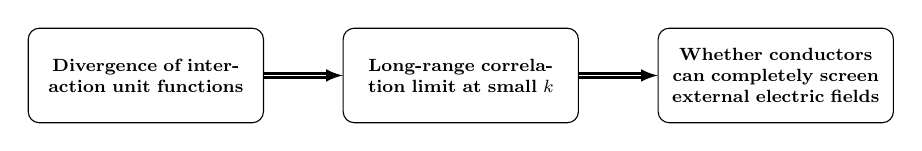
\begin{tikzpicture}[
				node style/.style={
					draw, 
					rounded corners, 
					align=center,
					minimum width=2.5cm,   
					minimum height=1.5cm,   
					font=\footnotesize,     
					text width=3.5cm,     
					fill=none
				},
				>=latex,
				scale=0.8,                 
				transform shape             
				]
				
				\node[node style] (node1) at (0,0) 
				{\textbf{Divergence of interaction unit functions}};
				
				\node[node style] (node2) at (5,0) 
				{\textbf{Long-range correlation limit at small $k$}};
				
				\node[node style] (node3) at (10,0)    
				{\textbf{Whether conductors can completely screen external electric fields}};
				
				\draw[->, thick, double] (node1) -- (node2);
				\draw[->, thick, double] (node2) -- (node3);
				
			\end{tikzpicture}
		\end{textblock*}
	\end{frame}
	%%%%%%%%%%%%%%%%%%%%%%%%%%%%%%%%%%%%%%%%%%%%%%%%%%%%%%%%%%%%%%%%%%%%%%%%%%%%%%%%
	\begin{frame}
		\frametitle{I . Virial Theorem in PBC  and Homogeneity}    	
		\footnotesize 
		
		\textbf{Virial Theorem:}
		\begin{equation*}
			P = k_B T\dfrac{1}{Z} \dfrac{\partial Z}{\partial V} , \quad Z =  \int_{V} \cdots \int_{V} e^{-\beta U} \, d\mathbf{r}_1 \dots d\mathbf{r}_N  
		\end{equation*}
		
		
		\begin{columns}[T]
			
			
			
			\begin{column}{0.5\textwidth}
				\centering
				\textbf{general case}
				\begin{equation*}
					U(\mathbf{r}_1, \dots , \mathbf{r}_N)  
				\end{equation*}
				\begin{equation*}
					P= \dfrac{N k_B T}{ V} + \dfrac{1}{3V} \langle \sum_i^N \mathbf{r}_i \cdot \mathbf{F}_i  \rangle  \label{eq:P=Nk_BT} 
				\end{equation*}
			\end{column}% 
			
			\begin{column}{0.5\textwidth}
				\centering
				\textbf{under PBC}  				
				\begin{equation*}
					U(\mathbf{r}_1, \dots , \mathbf{r}_N)  \Rightarrow  U(\{ \mathbf{r}_i \}, V)
				\end{equation*}
				\begin{equation*}
					P 
					= \dfrac{Nk_BT}{V} + \dfrac{1}{3V} \bigg{\langle}  \sum_i^N \mathbf{r}_i \cdot \mathbf{F}_i \bigg{\rangle}  - \bigg{\langle}  \dfrac{\partial U(\{ \mathbf{r}_i \}, V)}{\partial V}  \bigg{\rangle} 
				\end{equation*} 
			\end{column}% 
		\end{columns} 
		
		\vspace{10pt}
		Starting from the complete electrostatic potential $u_{\text{pair}}(\mathbf{r})$:
		
		\begin{equation*}
			P = \dfrac{Nk_BT}{V} -  \bigg{\langle} \dfrac{\partial U}{\partial V} \bigg{\rangle}   = \dfrac{Nk_BT}{V} +  \bigg{\langle}  \dfrac{U}{3V} \bigg{\rangle} 
		\end{equation*}
		Originating from the $L^{-1}$-homogeneity of all length quantities in $ u_{\mathrm{pair}} $.
		
		\begin{equation*}
			u_{\text{pair}}(\mathbf{r}) = \frac{1}{r} + \sum_{\mathbf{n} \ne 0} \left( \frac{1}{|\mathbf{r} + \mathbf{nL}|} - \frac{1}{|\mathbf{nL}|} \right)
		\end{equation*}
		
		
		\noindent\rule{\textwidth}{0.4pt}
		\centering
		\small
		\textbf{Therefore, this relation serves as the strict criterion for pressure in periodic systems.} 
	\end{frame}
	%%%%%%%%%%%%%%%%%%%%%%%%%%%%%%%%%%%%%%%%%%%%%%%%%%%%%%%%%%%%%%%%%%%%%
	\begin{frame}
		\frametitle{I . Virial Theorem in PBC and Homogeneity}    	
		\footnotesize 
		
		\textbf{Ewald interaction class :}
		\begin{align*}
			&u_{\text{pair}}^{ib, shape}(\mathbf{r})  : \text{  a rearrangement of    } \quad   u_{\text{pair}}(\mathbf{r}) \qquad \text{satisfies} \\
			&u_{\text{pair}}^{tf}(\mathbf{r})  : \text{  a rearrangement of    } \quad   u_{\text{pair}}(\mathbf{r}) - u^{ib}_{\text{pair}}(\mathbf{r}) \qquad \text{satisfies}
		\end{align*}
		
		\textbf{aa:}
		\begin{equation*}
			u_{\text{pair}}^{aa} = 
			\bigg{(} \dfrac{1}{r} +  \dfrac{r^2}{2r_m^3} - \dfrac{3}{2r_m}\bigg{)} + \sum_{\mathbf{n} \ne 0 }\bigg{(}\dfrac{1}{|\mathbf{r} + \mathbf{nL}|} +  \dfrac{|\mathbf{r} + \mathbf{nL}|^2}{2r_m^3} - \dfrac{3}{2r_m} \bigg{)} \qquad \text{satisfies}
		\end{equation*}
		
		\textbf{zm, 1:}
		\begin{equation*}
			u_{\text{pair}}^{zm, 1} = 
			\bigg{(} \dfrac{1}{r} +  \dfrac{r^2}{2r_c^3} - \dfrac{3}{2r_c}\bigg{)} + \sum_{\mathbf{n} \ne 0 }\bigg{(}\dfrac{1}{|\mathbf{r} + \mathbf{nL}|} +  \dfrac{|\mathbf{r} + \mathbf{nL}|^2}{2r_c^3} - \dfrac{3}{2r_c} \bigg{)},  \qquad \text{violates}
		\end{equation*}
		
		\begin{center}
			difference: $r_m \propto L^{-1}$ , $r_c$ fixed 
		\end{center}
		
		
		\textbf{Thus, any $r$-space cutoff must $\propto L^{-1}$; \\
			otherwise, pressure artifacts arise, as seen in Zero-Multipole\footnotemark[10] .}
		
		\footnotetext[10]{H. Wang, X. Gao, and J. Fang, \textit{J. Chem. Theory Comput.} \textbf{12}, 5596--5608 (2016).}
	\end{frame}
	%%%%%%%%%%%%%%%%%%%%%%%%%%%%%%%%%%%%%%%%%%%%%%%%%%%%%%%%%%%%%%%%%%%%%%%%%%%%
	\begin{frame}
		\frametitle{I . Virial Theorem in PBC and Homogeneity}    	
		\footnotesize 
		\vspace{-2cm}
		Pressure correction in one-component plasma :
		\begin{equation*}
			U^{corr} = -\dfrac{\pi \bigg{(}\sum_{i=1}^N q_i \bigg{)}^2}{2\alpha^2  V} , \qquad 
			P^{corr} = -\bigg{\langle}  \dfrac{\partial U^{corr}}{\partial V} \bigg{\rangle} 
		\end{equation*}
	    originates from the neutralizing background (the \textbf{Jellium}) via $\text{erfc}(\alpha r)/r$.

		\begin{equation*}
			U^{corr} \quad \text{is a part of} \quad \dfrac{1}{2} \sum_{i< j} q_iq_j u_{\text{pair}}(\mathbf{r}_{ij}) - E_{\text{traditional Ewald}}
		\end{equation*}
		
		The neutralizing background is a non-physical entity, a byproduct of the Ewald construction.
		
		
		\begin{textblock*}{8cm}(1cm,6.5cm)  
			\textbf{Third property-form link: } \\  [5pt]
			
			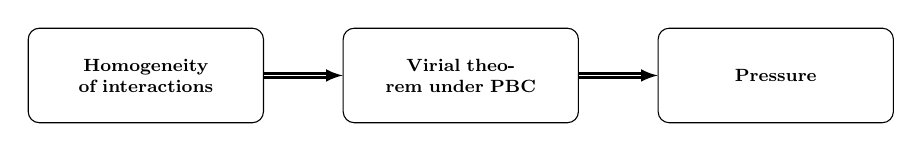
\begin{tikzpicture}[
				node style/.style={
					draw, 
					rounded corners, 
					align=center,
					minimum width=2.5cm,   
					minimum height=1.5cm,   
					font=\footnotesize,     
					text width=3.5cm,     
					fill=none
				},
				>=latex,
				scale=0.8,                 
				transform shape             
				]
				
				\node[node style] (node1) at (0,0) 
				{\textbf{Homogeneity of interactions}};
				
				\node[node style] (node2) at (5,0) 
				{\textbf{Virial theorem under PBC}};
				
				\node[node style] (node3) at (10,0)    
				{\textbf{Pressure} };
				
				\draw[->, thick, double] (node1) -- (node2);
				\draw[->, thick, double] (node2) -- (node3);
				
			\end{tikzpicture}
		\end{textblock*}
	\end{frame}
	%%%%%%%%%%%%%%%%%%%%%%%%%%%%%%%%%%%%%%%%%%%%%%%%%%%%%%%%%%%%%%%%%%%%%%%%%%%%%%%%%
	\begin{frame}
		\frametitle{I . Summary}
		\footnotesize
		\centering
		
		\vspace{-1cm}
		\begin{center}
			\textbf{A Unified Theoretical Framework}
		\end{center}
		
		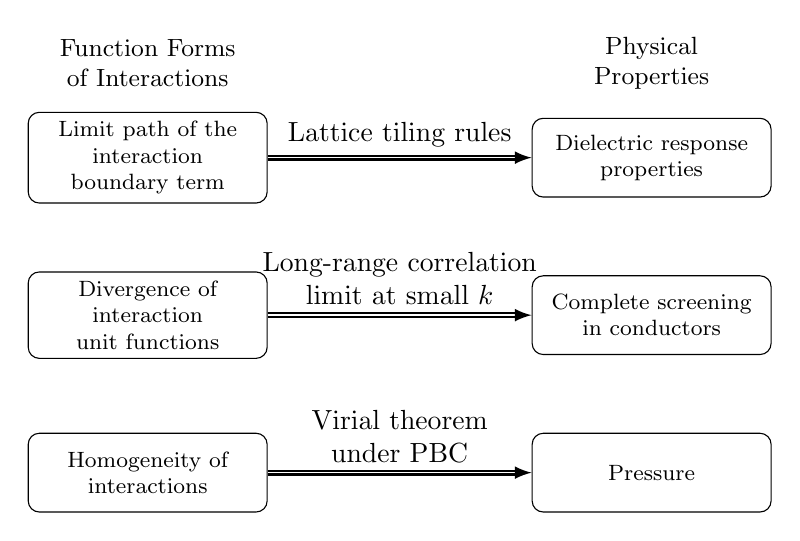
\begin{tikzpicture}[
			node style/.style={
				draw, 
				rounded corners, 
				align=center,
				minimum width=3cm,   
				minimum height=1cm,   
				font=\footnotesize,     
				text width=2.8cm,     
				fill=none
			},
			>=latex,
			scale=0.8
			]
			
			\node[align=center, font=\small] at (0,4) {Function Forms\\of Interactions};
			
			\node[node style] (L1) at (0,2.5) 
			{Limit path of the\\interaction boundary term};
			\node[node style] (L2) at (0,0) 
			{Divergence of\\interaction unit functions};
			\node[node style] (L3) at (0,-2.5) 
			{Homogeneity of\\interactions};
			
			\node[align=center, font=\small] at (8,4) {Physical\\Properties};
			\node[node style] (R1) at (8,2.5) 
			{Dielectric response\\properties};
			\node[node style] (R2) at (8,0) 
			{Complete screening\\in conductors};
			\node[node style] (R3) at (8,-2.5) 
			{Pressure};
			
			\draw[->, thick, double] (L1) -- node[above, pos=0.5] {Lattice tiling rules} (R1);
			\draw[->, thick, double] (L2) -- node[above, pos=0.5, align=center] {Long-range correlation\\limit at small $k$} (R2);
			\draw[->, thick, double] (L3) -- node[above, pos=0.5, align=center] {Virial theorem\\under PBC} (R3);
			
			
		\end{tikzpicture}
	\end{frame}
	%%%%%%%%%%%%%%%%%%%%%%%%%%%%%%%%%%%%%%%%%%%%%%%%%%%%%%%%%%%%%%%%%%%%%%%%%%%%%%   
	
	
	
	
	
	
	
	
	
	
	
	
	
	
	
	
	
	
	
	
	
	
	
	
	
	
	
	%%%%%%%%%%%%%%%%%%%%%%%%%%%%%%%%%%%%%%%%%%%%%%%%%%%%%%%%%%%%%%%%%5	
	\begin{frame}
		\frametitle{II. A PME without Systematic Error}
		
		Building upon Ewald's concept and focusing on computational efficiency has led to:
		\vspace{0.6cm}
		
		\begin{itemize}
			\item A family of particle-mesh methods (PME, SPME, PPPM).
			\vspace{0.3cm}
			\item Yet, theoretical inaccuracies and technical issues (e.g., global FFT communication) limit larger-scale simulations (e.g., D. E. Shaw's Anton).
		\end{itemize}
		
		\vspace{0.6cm}
		Thus, analyzing and eliminating these errors is essential.
	\end{frame}
	%%%%%%%%%%%%%%%%%%%%%%%%%%%%%%%%%%%%%%%%%%%%%%%%%%%%%%%%%%555
	
	\begin{frame}
		\frametitle{II. Particle Mesh Ewald }
		\footnotesize 
		
		\begin{textblock*}{10cm}(1cm,1.0cm)  
			PME ($\mathscr{O}(N\lg N)$ ) is a fast algorithm for Ewald summation ($\mathscr{O}(N^2)$)\footnotemark[11]{\textsuperscript{,}}\footnotemark[12]
		\end{textblock*}
		
		\begin{textblock*}{5cm}(7.8cm,2cm)  
			\begin{figure}[h]
				\centering
				\includegraphics[width=0.7\linewidth]{./figure/mesh/mesh.png}	
			\end{figure}
		\end{textblock*}
		
		
		\begin{textblock*}{6.2cm}(1cm,1.5cm)
			
			\begin{equation*}
				E^{k}=\dfrac{1}{2V} \sum_{\mathbf{k}\ne 0} \dfrac{4\pi}{k^2}e^{-\frac{k^2}{4\alpha^2}} \bigg{(}\sum_{i=1}^{N} q_ie^{i\mathbf{k}\mathbf{r}_{i}} \bigg{)} \bigg{(}\sum_{j=1}^{N} q_je^{-i\mathbf{k}\mathbf{r}_{j}} \bigg{)} 
			\end{equation*}
			
			Interpolating $e^{ikx}$ = charge interpolation + FFT :
			\begin{align}
				q_je^{i k_1x_j} \approx& \sum_{n_1=0}^{K_1-1} q_j W_p(x_j - n_1\dfrac{L_x}{K_1}) e^{ik_1 n_1 \frac{L_x}{K_1}} \notag \\
				=& \text{FFT1D}[ q_j W_p(x_j - n_1\dfrac{L_x}{K_1}) ](m_1) \notag 
			\end{align}
			
			$W_p$: interpolation coefficient of order $p$.
			
		\end{textblock*}
		
		\begin{textblock*}{6.2cm}(1cm,6.5cm)
			\begin{align*}
				E^{k}_{\text{PME}}=\dfrac{1}{2} \sum_{m_1 = 0}^{K_1-1} \sum_{m_2 = 0}^{K_2-1} \sum_{m_3 = 0}^{K_3-1}\dfrac{1}{V}\dfrac{4\pi}{k^2}e^{-\frac{k^2}{4\alpha^2}} \text{FFT3D}[Q](m_1, m_2, m_3)\cdot
				\text{FFT3D}[Q](-m_1, -m_2, -m_3) \notag 
			\end{align*}
		\end{textblock*}
		
		\footnotetext[11]{T. Darden and L. Pedersen, J. Chem. Phys. \textbf{98}, 10089(1993) }
		\footnotetext[12]{U. Essmann and L.G. Pedersen, J. Chem. Phys. \textbf{103}, 8577(1995)}
	\end{frame}
	
	
	
	
	%%%%%%%%%%%%%%%%%%%%%%%%%%%%%%%%%%%%%%%%%%%%%%%%%%%%%%%%%%%%%%%%%%%5
	\begin{frame}
		\frametitle{II.  Truncation Error and It's Elimination }
		\footnotesize 
		
		\begin{textblock*}{8cm}(1cm,1.5cm)
			
			Wavevector cutoff in interactions couples to
			mesh  size $K_1 \times K_2 \times K_3$:
			
			\begin{equation*}
				u^{k}(\mathbf{r}) = \dfrac{1}{V} \sum_{\mathbf{k} \in \mathbf{k}_{\text{cut}}} \dfrac{4\pi}{k^2} e^{-\dfrac{k^2}{4\alpha^2}} e^{i\mathbf{k}\cdot\mathbf{r}} 
			\end{equation*}
			
			Wavevector :
			\begin{equation*}
				\mathbf{k}(m_1\dfrac{2\pi}{L_x}, m_2\dfrac{2\pi}{L_y}, m_3\dfrac{2\pi}{L_z}), \quad 
				\dfrac{K}{2} \ge m \le \dfrac{K}{2} -1 
			\end{equation*}
			
			So:
			\begin{equation*}
				u^k(\mathbf{r})(\text{small } K_1 \times K_2 \times K_3) \text{ differs from } u^k(\mathbf{r})(\text{large } K_1 \times K_2 \times K_3)
			\end{equation*}
			
			This is the truncation error in PME.
		\end{textblock*}
		
		\begin{textblock*}{8cm}(6cm,2cm)  
			\begin{figure}[h]
				\centering
				\includegraphics[width=0.6\linewidth]{./figure/upair_Kcut/upair_Kcut.pdf}	
			\end{figure}
		\end{textblock*}
		
		\vspace{6cm} 
		
		
		\noindent\rule{\textwidth}{0.4pt}
		\centering
		\small
		\textbf{Truncation error is the main reason that restricts mesh size to satisfy $L/K \approx 1 \si{\angstrom}$ .} 		
	\end{frame}
	%%%%%%%%%%%%%%%%%%%%%%%%%%%%%%%%%%%%%%%%%%%%%%%%%%%%%%%%%%%%%%%%%%%%%%%%%	
	\begin{frame}
		\frametitle{II.  Truncation Error and Its Elimination}
		\footnotesize 
		\begin{textblock*}{10cm}(1cm,1cm)
			Decoupling wavevector cutoff range from mesh size:
			\begin{equation*}
				u^{k}_{K'}(\mathbf{r}) = \dfrac{1}{V} \sum_{\mathbf{k} \in \mathbf{K}'} \dfrac{4\pi}{k^2} e^{-\dfrac{k^2}{4\alpha^2}} e^{i\mathbf{k}\cdot\mathbf{r}} 
			\end{equation*}
			
			$K'$ is enough to make $u_{K'}^k$ converge. Corresponding non-trunc PME:
			
			\vspace{-10pt}
			\begin{equation*}
				E_{k}^{\text{PME}}=\dfrac{1}{2} \sum_{m_1 = 0}^{K_1-1} \sum_{m_2 = 0}^{K_2-1} \sum_{m_3 = 0}^{K_3-1} \bigg{(}\text{FFT3D}[\dfrac{1}{K_1'K_2'K_3'}u_{K'}] \bigg{)} \text{FFT3D}[Q](\mathbf{m})\cdot 
				\text{FFT3D}[Q](-\mathbf{m}) 
			\end{equation*}
		\end{textblock*}
		
		\begin{textblock*}{6cm}(1cm,4.8cm) 
			\begin{table}
				\caption*{charge exactly on grid}
				\centering
				\begin{tabular}{ccc}
					\toprule
					\multirow{2}{*}{$K_1\cdot K_2 \cdot K_3$} &
					\multicolumn{2}{c}{$E_k^{\mathrm{PME}}(\mathrm{kJ/mol})$} \\
					\cmidrule{2-3}
					& ori-PME& non-PME \\ \midrule
					$16\cdot16\cdot16$ &441.5625& 745.7720 \\
					$32 \cdot 32 \cdot 32$&675.6669& 745.7720 \\ 
					$64\cdot 64 \cdot 64 $ &744.8545& 745.7720\\
					$ 128\cdot 128 \cdot 128 $ &745.7720 & 745.7720\\\bottomrule
				\end{tabular}
			\end{table}	
		\end{textblock*}	 
		
		
		
		\begin{textblock*}{5cm}(7cm,5cm)  
			\begin{figure}[h]
				\centering
				\includegraphics[width=\linewidth]{./figure/nontsig3/nontsig3.pdf}
				\caption*{simulation sampling}
			\end{figure}
		\end{textblock*}
		
		
	\end{frame}
	%%%%%%%%%%%%%%%%%%%%%%%%%%%%%%%%%%%%%%%%%%%%%%%%%%%%%%%%%%%%%%5	
	\begin{frame}
		\frametitle{II.  Artifact Error and It's Elimination}
		\footnotesize 
		
		
		Interpolating each single charge produces artifacts, 
		where part of the interactions are redundant (but not all).
		
		\begin{textblock*}{5cm}(1cm,2cm)  
			\begin{figure}[h]
				\centering
				\includegraphics[width=0.6\linewidth]{./figure/mesh/mesh_i.png}
				\caption*{Blue points are artifacts}
			\end{figure}
		\end{textblock*}
		
		
		
		\begin{textblock*}{6cm}(6cm,2cm)  
			
			
			\begin{figure}
				\centering
				\includegraphics[width=0.9\linewidth]{./figure/u_pair_p2/u_pair_p2.pdf}
				\vspace{-5pt}
				\caption*{\qquad $\mathbf{r}_1 = 0$, $\mathbf{r}_2 = (0,0,r)$}
			\end{figure}
		\end{textblock*}
		
		\vspace{4.6cm} 
		Defining PME interactions in two-charge systems :
		\begin{equation*}
			u_{\text{PM}}^k (\mathbf{r}_1, \mathbf{r}_2) =  \dfrac{E^{k}_{\text{non-trunc}}(\mathbf{r}_1, \mathbf{r}_2)}{q_1q_2}
		\end{equation*}
		
		This is the artifact error in PME.
		
		\noindent\rule{\textwidth}{0.4pt}
		\centering
		\small
		\textbf{Artifact error cause regular oscillations in PME interactions.}
	\end{frame}
	%%%%%%%%%%%%%%%%%%%%%%%%%%%%%%%%%%%%%%%%%%%%%%%%%%%%%%%%%%%%%%%%%%%%%%%%%%%%%%%	
	\begin{frame}
		\frametitle{II.  Artifact Error and It's Elimination}
		\footnotesize 
		
		
		Directly removing the redundant interaction energy yields non-artifact PME, but the difficulty lies in that each single point charge's artifact system is non-electroneutral.
		
		\begin{textblock*}{6cm}(0.2cm,2cm)  
			\begin{figure}
				\centering
				\includegraphics[width=0.9\linewidth]{./figure/nonau_pair_p2/nonau_pair_p2.pdf}
			\end{figure}
		\end{textblock*}
		
		
		\begin{textblock*}{6cm}(6.2cm,2cm)  
			\begin{figure}[h]
				\centering
				\includegraphics[width=0.9\linewidth]{./figure/nonasig3/nonasig3.pdf}
			\end{figure}
		\end{textblock*}
		
		\vspace{4cm}
		
		Calculating $E_i$ via non-neutral Ewald/PME : 
		\begin{equation*}
			E^{k}_{\text{non-artif}}  =	E^{k}_{\text{non-trunc}} - \sum_{i=1}^N E^{k}_{i}(\text{$q_i$ coordinates relative to the grid})
		\end{equation*}
		
		\vspace{0cm}
		Corresponding to non-artif PME. \\ [5pt]
		Higher-order interpolation follows the same principle as linear but is more complex.
	\end{frame}
	%%%%%%%%%%%%%%%%%%%%%%%%%%%%%%%%%%%%%%%%%%%%%%%%%%%%%%%%%%%%%%%%%%%%%%%%%%
	\begin{frame}
		\frametitle{II. Fitting Error of Interactions and It's Elimination}  
		\footnotesize 
		
		Perspective shift: from discrete charge interactions to original charge interactions
		
		\begin{equation*}
			u_{\mathrm{PM}}^{\text{non-artif}}(\mathbf{r}_1, \mathbf{r}_2)
			= \sum_{\mathbf{m}} W_p(\mathbf{r}_1, \mathbf{m})  \sum_{\mathbf{n}} W_p(\mathbf{r}_2, \mathbf{n}) \cdot u_{\text{pair}}(\mathbf{r}_{\mathrm{grid}}(\mathbf{m}) - \mathbf{r}_{\mathrm{grid}}(\mathbf{n})  )  \label{eq:fiterror}
		\end{equation*}
		
		which deviates from exact results and depends independently on $\mathbf{r}_1$ and $\mathbf{r}_2$.
		
		\begin{textblock*}{6cm}(0.2cm,3cm)  
			\begin{figure}
				\centering
				\includegraphics[width=0.9\linewidth]{./figure/u_fiterror_p2/u_fiterror_p2.pdf}
				\vspace{-5pt}
				\caption*{\qquad $\mathbf{r}_1=(0,0,0)$, $\mathbf{r}_2=(0,0,r)$}
			\end{figure}
		\end{textblock*}
		
		
		\begin{textblock*}{6cm}(6.2cm,3cm)  
			\begin{figure}[h]
				\centering
				\includegraphics[width=0.9\linewidth]{./figure/u_fiterror_p2_diffr1/u_fiterror_p2_diffr1.pdf}
				\vspace{-5pt}
				\caption*{\qquad varying $\mathbf{r}_1$}
			\end{figure}
		\end{textblock*}
		
		
		\vspace{4.5cm} 
		
		This is the fitting error of interactions.  
		
		Meanwhile, the $r$-space interaction of the original charge remains unchanged.
		
		\noindent\rule{\textwidth}{0.4pt}
		\centering
		\small
		\textbf{Fitting error causes Ewald's splitting of $1/r$ to be no longer complete.}     
	\end{frame}
	%%%%%%%%%%%%%%%%%%%%%%%%%%%%%%%%%%%%%%%%%%%%%%%%%%%%%%%%%%%%%%
	\begin{frame}
		\frametitle{II. Fitting Error of Interactions and It's Elimination}  
		\footnotesize 
		
		Eliminate all unphysical dependencies through "translation-rotation averaging":
		\begin{equation*}
			\langle \Delta u \rangle_{sp} = 
			= \dfrac{1}{2\pi^2 \Omega} \int_{\Omega} d\mathbf{r}_1 \, \int_{0}^{\pi}d\theta \, \int_{0}^{2\pi} d\varphi \, [u_{\mathrm{PM}}^{\mathrm{non-artif}}-u_{\text{pair}}](\mathbf{r}_1, \theta, \varphi) 
		\end{equation*}
		Merge $\langle \Delta u \rangle_{sp}$ into the original $r$-space interaction to ensure complete splitting.
		
		\begin{textblock*}{6cm}(0.2cm,3.2cm)  
			\begin{figure}
				\centering
				\includegraphics[width=0.9\linewidth]{./figure/u_fiterror_p2_ava/u_fiterror_p2_ava.pdf}
			\end{figure}
		\end{textblock*}
		
		
		\begin{textblock*}{6cm}(6.2cm,3.2cm)  
			\begin{figure}[h]
				\centering
				\includegraphics[width=0.9\linewidth]{./figure/nonssig3/nonssig3.pdf}
				\vspace{-5pt}
				\caption*{$L_x = L_y = L_z = 100 \si{\angstrom}$}
			\end{figure}
			
		\end{textblock*}
		
		
		\vspace{4.5cm} 
		non-sys PME: accurate at $16\times 16\times 16$ (original PME requires $128\times 128\times 128$) \\  [5pt]
		
		
		Remaining \textbf{unbiased noise} requires $\mathscr{O}(N^2)$, conflicting with $\mathscr{O}(N\log N)$. 
		
		Thus, we consider the unbiased noise as the \textbf{minimal cost} of PME calculation.
		
		
	\end{frame}
	%%%%%%%%%%%%%%%%%%%%%%%%%%%%%%%%%%%%%%%%%%%%%%%%%%%%
	\begin{frame}
		\frametitle{II. Summary}
		\footnotesize
		\centering
		
		\vspace{-0.5cm}
		\begin{center}
			\textbf{A PME Without Systematic Errors}
		\end{center}
		
		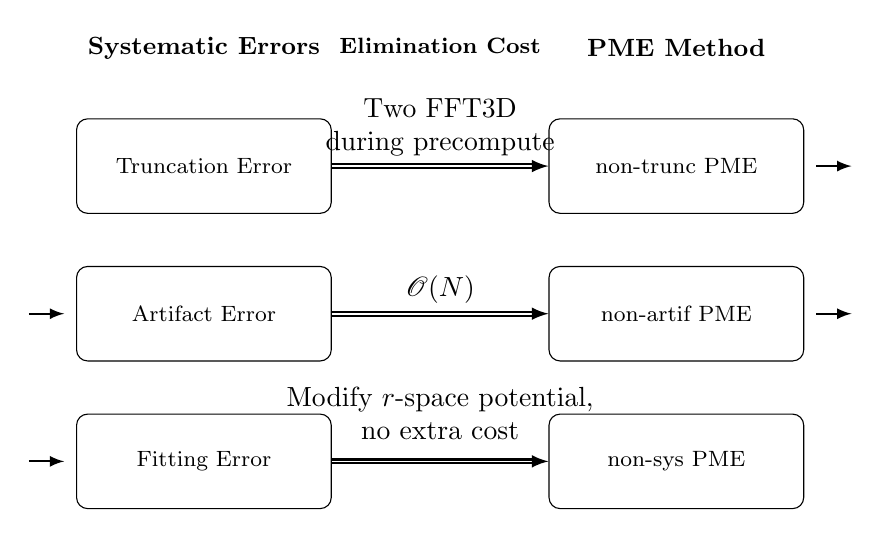
\begin{tikzpicture}[
			node style/.style={
				draw, 
				rounded corners, 
				align=center,
				minimum width=3.2cm,   
				minimum height=1.2cm,   
				font=\footnotesize,
				text width=3cm,
				fill=none
			},
			>=latex,
			scale=0.75
			]
			
			% Left side: Three Errors
			\node[align=center, font=\small] at (0,4.5) {\textbf{Systematic Errors}};
			\node[node style] (L1) at (0,2.5) {Truncation Error};
			\node[node style] (L2) at (0,0) {Artifact Error};
			\node[node style] (L3) at (0,-2.5) {Fitting Error};
			
			% Right side: Three PME versions
			\node[align=center, font=\small] at (8,4.5) {\textbf{PME Method}};
			\node[node style] (R1) at (8,2.5) {non-trunc PME};
			\node[node style] (R2) at (8,0) {non-artif PME};
			\node[node style] (R3) at (8,-2.5) {non-sys PME};
			
			% Main arrows connecting left and right
			\draw[->, thick, double] (L1) -- node[above, yshift=1.3cm] {\footnotesize \textbf{Elimination Cost}} node[above, pos=0.5, align=center] {Two FFT3D \\during precompute} (R1);
			\draw[->, thick, double] (L2) -- node[above, pos=0.5, align=center] {$\mathscr{O}(N)$} (R2);
			\draw[->, thick, double] (L3) -- node[above, pos=0.5, yshift=4pt, align=center] {Modify $r$-space potential,\\ no extra cost } (R3);
			
			% Rightward progression arrows on the LEFT side (only for L2 and L3)
			\draw[->, thick] (L2.west) ++(-0.8,0) -- ++(0.6,0);
			\draw[->, thick] (L3.west) ++(-0.8,0) -- ++(0.6,0);
			
			% Rightward progression arrows on the RIGHT side  
			\draw[->, thick] (R1.east) ++(0.2,0) -- ++(0.6,0);
			\draw[->, thick] (R2.east) ++(0.2,0) -- ++(0.6,0);
			
		\end{tikzpicture}
		
		Non-sys PME: ~100× faster (~90× theoretical) via mesh sparsification, with significantly reduced memory. 
		
		\vspace{6pt}
		
		Furthermore, we argue that the conflict between \textbf{momentum} and \textbf{energy} conservation in PME is irreconcilable.
	\end{frame}
	%%%%%%%%%%%%%%%%%%%%%%%%%%%%%%%%%%%%%%%%%%%%%%%%%%%%%%%%%%%%%%%%%%%%%%%%%%
	
	
	\begin{frame}
		\frametitle{III. Toward MLFFs without Systematic Error} 
		\footnotesize 
		
		\begin{textblock*}{7cm}(1cm,1.6cm)  
			
			Map \textbf{local} environment to energy/forces
			\begin{equation*}		
				E_{\text{PBC}} = \sum_{i=1}^N E_{\text{vacuum}}(\mathbf{r}_i; r_c)
			\end{equation*}

			This inherently contradicts long-range electrostatics.
		\end{textblock*}
		
		\vspace{3.8cm}
		Therefore, long- and short-range interactions must be separated in ML training data.
		
		
		\begin{textblock*}{7cm}(2cm,6.2cm)  
			With rigorous separation, \\
			ML is already sufficiently powerful \\
			(Accuracy: $10^{-1}$ meV/Å). \\
		\end{textblock*}
		
		
		\begin{textblock*}{5cm}(8cm,1.3cm)
			\begin{figure}
				\centering
				\includegraphics[width=0.6\linewidth]{./figure/qiu.png}
			\end{figure}
		\end{textblock*}
		
		% Bottom-right: Table
		\begin{textblock*}{6cm}(7cm,5cm)
			\begin{table}[h]
				\centering    		
				\resizebox{0.75\textwidth}{!}{%	
					\begin{threeparttable}     
						\caption*{Drude Model}		
						\begin{tabular}{*{3}{c}}
							\toprule
							\multirow{2}{*}{ML} & \multicolumn{2}{c}{$\langle|F_i^{\mathrm{ML}} - F_i|\rangle$($\mathrm{meV}/\si{\angstrom}$)} \\
							\cmidrule(lr){2-3}
							& Na-core & Cl-core \\ 
							\midrule
							exact-BPNN & $1.713\times 10^{-7}$ & $1.713\times 10^{-7}$\\ 
							DPMD-short & $3.695\times 10^{-1}$ & $4.238\times 10^{-1}$\\ 
							DPMD-full & $22.086$ & $18.946$ \\
							\bottomrule
						\end{tabular}
						\begin{tablenotes}
							\small
							\item First two lines: short-range forces only
							\item Last line: total force
						\end{tablenotes}
				\end{threeparttable}}
			\end{table}
		\end{textblock*}
		
		\vspace{3.2cm}
		\noindent\rule{\textwidth}{0.4pt}
		\centering
		\small
		\textbf{Thus, correct separation of long-range and short-range interactions is key.}   
	\end{frame}
	
	%%%%%%%%%%%%%%%%%%%%%%%%%%%%%%%%%%%%%%%%%%%%%%%%%55
		\begin{frame}
		\frametitle{III. Toward MLFFs without Systematic Error} 
		\footnotesize
		
	    Current separation fails because:
	    \begin{itemize}
	    	\item \textit{ab initio} forces originate from delocalized electron clouds, not atom-centered point charges
	    	\item Separation replaces true density with point charges (nuclei + Wannier centers)
	    \end{itemize}
		
		\vspace{0.5cm}
		Therefore, rigorous separation must be based on precise atom-assignable electron density distribution.
		
		\vspace{0.4cm}
		Based on the same methodology as X-ray spectrum analysis:
		\begin{itemize}
			\item Solve bulk total X-ray spectrum and static structure factor
			\item Obtain atom-assignable density via inverse transform with physically constrained form factors
		\end{itemize}
		
		
		\vspace{0.8cm}
		\noindent\rule{\textwidth}{0.4pt}
		\centering
		\small
		\textbf{This enables rigorous long- and short-range separation in training data — a crucial step toward MLFFs without Systematic Error.}   
		

	\end{frame}

    %%%%%%%%%%%%%%%%%%%%%%%%%%%%%%%%%%%%%%%%%%%%%%%%%%%55
    \begin{frame}
    	\frametitle{III. Toward MLFFs without Systematic Error} 
    	\footnotesize
    	
    	In adiabatic dynamics, even without long-range interactions, systematic errors persist:
    	
    	\vspace{0.2cm}
    	\begin{itemize}
    		\item Electronic self-consistency is intrinsically global. Even in purely short-range systems, local equilibrium $\neq$ global equilibrium
    		\item In essence, this indirect correlation is also long-ranged
    	\end{itemize}
    	
    	\vspace{0.4cm}
    	Implication: Different local environments should exchange information when mapping to atomic forces — analogous to FFT's global communication.
    	
    	
    	
    	\vspace{0.8cm}
    	\noindent\rule{\textwidth}{0.4pt}
    	\centering
    	\small
    	\textbf{Therefore, the nonlocality of both long-range and indirect correlations is the primary source of systematic errors in MLFFs.}   
    	
    	
    	
    
    	
    \end{frame}
    %%%%%%%%%%%%%%%%%%%%%%%%%%%%%%%%%%%%%%%%%%%%%%%%%%%55
     
     
\end{document}